\documentclass[11pt]{article}
\usepackage[a4paper,margin=0.82in,top=0.72in,bottom=0.70in]{geometry}
\usepackage[T1]{fontenc}
\usepackage{lmodern}
\usepackage{microtype}
\usepackage{amsmath,amssymb,mathtools}
\usepackage{graphicx}
\usepackage{booktabs}
\usepackage{caption}
\usepackage{enumitem}
\usepackage{fancyhdr}
\usepackage{xcolor}
\usepackage[hidelinks]{hyperref}
\usepackage{titlesec}
\captionsetup{font=small,labelfont=bf}
\setlength{\parindent}{1.2em}
\setlength{\parskip}{0pt}
\setlist{nosep,leftmargin=1.5em}
\titleformat{\section}{\large\bfseries}{\thesection.}{0.55em}{}
\titleformat{\subsection}{\normalsize\bfseries}{\thesubsection}{0.55em}{}
\titlespacing*{\section}{0pt}{1.2em}{0.35em}
\titlespacing*{\subsection}{0pt}{0.9em}{0.25em}
\pagestyle{fancy}
\fancyhf{}
\fancyhead[C]{\footnotesize\color{gray}\textsc{Stable Principal Subspaces and Prediction}}
\fancyfoot[C]{\thepage}
\renewcommand{\headrulewidth}{0pt}
\setlength{\headheight}{14pt}
\begin{document}
\thispagestyle{plain}
\begin{center}
{\LARGE When Stable Principal Subspaces Fail Prediction\par}
\vspace{0.35em}
{\large An Empirical Study of Eigengap-Based Rank Selection\par}
\vspace{1.3em}
{\normalsize Yuva $\cdot$ Technical note $\cdot$ October 2026\par}
\end{center}
\vspace{1.2em}
\begin{abstract}
Stability-based and prediction-based methods for choosing the number of principal components answer different questions, and they are known to disagree when the predictive signal lies in low-variance components. This note quantifies when that disagreement occurs and what it costs, in a fully controlled synthetic setting: six features, a spiked covariance spectrum with an eigengap after the third component, and a linear response whose signal lies along a single chosen principal direction. Across 72 conditions (sample size $\times$ eigengap size $\times$ signal location) and 200 seeds per condition, we compare a bootstrap subspace-stability selector with cross-validated principal component regression (PCR). The cost of disagreement is governed almost entirely by the signal's position relative to the eigengap. When the signal lies beyond the gap, a larger gap and larger sample make stability-based selection more geometrically reliable and, at the same time, make its predictive failure more consistent: with a large gap and $n\geq 60$, the stability-selected model loses more than half of the signal variance in 99.9\% of runs, and on average all of it (mean excess error 1.00, with signal variance 1). The pattern holds when the signal lies in PC 4 or 5, where both rules can select a rank that retains it, so it is not produced by the stability rule's exclusion of rank 6. When the signal lies before the gap, the methods still disagree in 31--86\% of runs, with little or no predictive cost. The excess test error is approximately equal to the variance of the discarded signal. The underlying mechanisms are established; the contribution is the controlled, quantitative characterisation of the trade-off between geometric stability and predictive loss under the stated conditions.
\end{abstract}
\section{Question and positioning}

Principal component regression (PCR) needs a rank k. Two broad families of selection rules exist. Stability-based rules choose the k whose principal subspace is least sensitive to perturbation or resampling of the data (Besse, 1992; Song \& Shin, 2018). Prediction-based rules choose k by cross-validation (CV); here we use CV of the regression error itself, a long-studied choice for PCR (Shin \& Tanaka, 1996). Neither strategy is new. The two differ in kind: stability selection never looks at the response y, while PCR-CV does.\par

That an unsupervised criterion can discard predictive components is long established. Jolliffe (1982) showed that low-variance components can carry the regression signal, Hadi \& Ling (1998) showed that PCR can miss the predictive information entirely, and Artigue \& Smith (2019) used theoretical examples and Monte Carlo simulation to show how selecting high-variance components damages prediction. The question here is therefore narrower and quantitative:\par

\begin{quote}\itshape\centering Under which combinations of sample size, eigengap size and signal location do the two rules consistently disagree, and how much test error does the disagreement cost?\end{quote}

What this note adds is a direct comparison of the two rules across jointly controlled eigengaps, signal locations and sample sizes, with disagreement frequency and excess prediction loss reported separately. Within that comparison, the most specific observation is that stronger eigenvalue separation makes stability selection more consistent while making its predictive failure more systematic when the signal lies outside the selected subspace. This is a modest empirical characterisation of established mechanisms, not a new algorithm or theorem; Section 7 states what the literature check did and did not establish.\par

\section{Experimental setup}

\subsection{Data generator}

Features: $p=6$. The covariance matrix is $\Sigma=Q\operatorname{diag}(\boldsymbol\lambda)Q^{\mathsf T}$, where $Q$ is a random orthogonal matrix drawn independently for each seed (obtained from the QR decomposition of a Gaussian matrix). The spectrum has an eigengap after the third component:

\begin{equation}
\boldsymbol\lambda \propto \bigl(1.2g,\,1.1g,\,1.0g,\,1.0,\,0.9,\,0.8\bigr),\qquad \sum_{i=1}^{6}\lambda_i=6.
\end{equation}

Thus $\lambda_3/\lambda_4=g$. The mild decay within each block keeps every principal direction identifiable. The response follows
\begin{equation}
y=X\beta+\varepsilon,\qquad \varepsilon\sim\mathcal N(0,\sigma^2),\qquad \beta=c\,q_j,
\end{equation}
where $\sigma=1$ and $q_j$ is the $j$th population principal direction. The coefficient $c$ is chosen so that $\operatorname{Var}(X\beta)=c^2\lambda_j=\mathrm{SNR}\,\sigma^2$, with $\mathrm{SNR}=1$ in every main-grid condition. Moving the signal between components therefore does not change its strength.

\subsection{Controlled variables}

\begin{itemize}

\item Sample size: n $\in$ \{30, 60, 120, 500\}.

\item Eigengap: g = $\lambda_3/\lambda_4$ $\in$ \{1.5 (small), 3 (medium), 10 (large)\}.

\item Signal location: j $\in$ \{1, \ldots{}, 6\}; $j\leq 3$ is 'before the gap', $j\geq 4$ is 'beyond the gap'.

\end{itemize}

This gives 4 $\times$ 3 $\times$ 6 = 72 conditions, each run with 200 seeds (14,400 datasets). Seeds are deterministic functions of (n, g, j, seed index).\par

\subsection{Rank-selection rules}

\textbf{Stability-based.} For each $k\in\{1,\ldots,5\}$, define
\begin{equation}
\mathcal I(k)=\frac{1}{B}\sum_{b=1}^{B}\frac{1}{2}\left\lVert\widehat P_k-\widehat P_k^{(b)}\right\rVert_F^2,
\end{equation}
with $B=50$ bootstrap resamples. Here $\widehat P_k$ projects onto the top-$k$ principal subspace of the full training sample, while $\widehat P_k^{(b)}$ is the corresponding bootstrap projector. The selected rank minimizes $\mathcal I(k)$. This criterion is in the spirit of Besse (1992) and Song \& Shin (2018), but is not an exact implementation of either method. Rank $k=6$ is excluded because the projector onto $\mathbb R^6$ is the identity and therefore cannot move.

\textbf{Consequence of the asymmetry.} The two rules therefore have different candidate sets: \{1, \ldots{}, 5\} for stability, \{1, \ldots{}, 6\} for CV. When the signal lies in PC 6, stability selection cannot retain it at any rank, so part of its failure there is guaranteed by construction, independently of the eigengap. Results for PC 6 are therefore reported separately from PC 4--5 (Section 4.3, Table 3).\par

\textbf{Prediction-based.} 5-fold CV of PCR test error on the training sample, for k $\in$ \{1, \ldots{}, 6\}. Centring, the PCA and the regression are refitted inside every training fold.\par

\subsection{Outcomes}

For each dataset we record both selected ranks, a disagreement indicator, and the test mean squared error (MSE) of PCR at each selected rank, fitted on the full training sample and evaluated on an independent test set of 2,000 points. The main cost measure is $\Delta$ = MSE($k_{\mathrm{stability}}$) - MSE($k_{\mathrm{CV}}$). Because the signal variance is 1, $\Delta\approx 1$ means the stability-selected model has lost the entire signal.\par

\section{Validation checks}

\textbf{Selection rules.} The stability selector receives only X (its function signature is (X, rng)), and its choice was identical in 300/300 repeated calls without any access to y. The CV selector receives only the training sample. Absence of leakage rests on the code itself: fold indices are drawn from the training sample only, the PCA and regression are refitted inside each training fold, and the independent test set is generated separately and used only after both ranks have been selected. As an additional sanity check (not a proof), CV on pure-noise targets favoured small ranks ($k=1$ in 107/200 runs, $k=6$ in 8/200), as expected without leakage.\par

\textbf{Error decomposition.} If the excess error is the lost signal, $\Delta$ should equal $\mathrm{SNR}\,\sigma^2$ and scale with both. We reran one beyond-the-gap cell ($n=500$, large gap, $j=5$, 100 seeds) at five settings (Table 1). The excess matched $\mathrm{SNR}\,\sigma^2$ to within 4\% in every case, and the stability-selected model's MSE equalled the total variance of y: it predicts no better than the mean.\par

\begin{table}[!htbp]
\centering
\caption{Excess test MSE equals the signal variance ($n=500$, large gap, signal on PC 5; stability selected $k=3$ in 100\% of runs).}
\scriptsize
\setlength{\tabcolsep}{3.2pt}
\begin{tabular}{@{}lrrrrrr@{}}
\toprule
SNR & $\sigma$ & Expected $\mathrm{SNR}\,\sigma^2$ & MSE (stability) & MSE (CV) & $\operatorname{Var}(y)$ & Observed $\Delta$ \\
\midrule
1 & 1 & 1.00 & 2.013 & 1.021 & 1.995 & 0.992 \\
0.5 & 1 & 0.50 & 1.511 & 1.021 & 1.498 & 0.491 \\
2 & 1 & 2.00 & 3.018 & 1.021 & 2.992 & 1.997 \\
1 & 2 & 4.00 & 8.051 & 4.084 & 7.981 & 3.968 \\
0.25 & 2 & 1.00 & 5.046 & 4.084 & 4.999 & 0.962 \\
\bottomrule
\end{tabular}
\end{table}

\textbf{Theory.} Figure~3 uses two distinct theoretical references. For Gaussian data, the first-order perturbation approximation is
\begin{equation}
\mathbb E\left\lVert\widehat P_k-P_k\right\rVert_F^2\approx \frac{2}{n}\sum_{i\leq k<j}\frac{\lambda_i\lambda_j}{(\lambda_i-\lambda_j)^2}.
\end{equation}
This is an asymptotic approximation, not a bound (Anderson, 1963). The Davis--Kahan variant of Yu, Wang \& Samworth (2015) gives
\begin{equation}
\lVert\sin\Theta\rVert_F \leq \frac{2\min\{\sqrt{k}\lVert\widehat\Sigma-\Sigma\rVert_{\mathrm{op}},\,\lVert\widehat\Sigma-\Sigma\rVert_F\}}{\lambda_k-\lambda_{k+1}},\qquad\lVert\widehat P-P\rVert_F=\sqrt{2}\lVert\sin\Theta\rVert_F.
\end{equation}
This deterministic bound was evaluated for each sample and held in all 10,500 cases. The check confirms consistency with the theorem; it is not an additional empirical result.

\section{Results}

\subsection{Pilot: a spectrum without a gap}

A first version used a geometric spectrum ($\lambda_{k+1}/\lambda_k$ constant), i.e. no preferred gap. Stability selection then had no stable rank to find: across all conditions it chose $k=1$ in 38\% of runs and $k=5$ in 30\%, with $k=2$--4 in the remaining 32\%. The two extremes are symmetric for a geometric spectrum: the eigenvalue pairs split by $k=1$ and by $k=5$ have identical ratios, so their predicted instabilities coincide. Disagreement with CV was 86\% overall and the eigengap variable had no systematic effect. The covariance spectrum is therefore not a nuisance detail: without a real gap, stability selection is close to arbitrary. The main experiment uses the spiked spectrum of Section 2.1.\par

\subsection{The boundary: signal location relative to the gap}

\begin{figure}[!htbp]
\centering
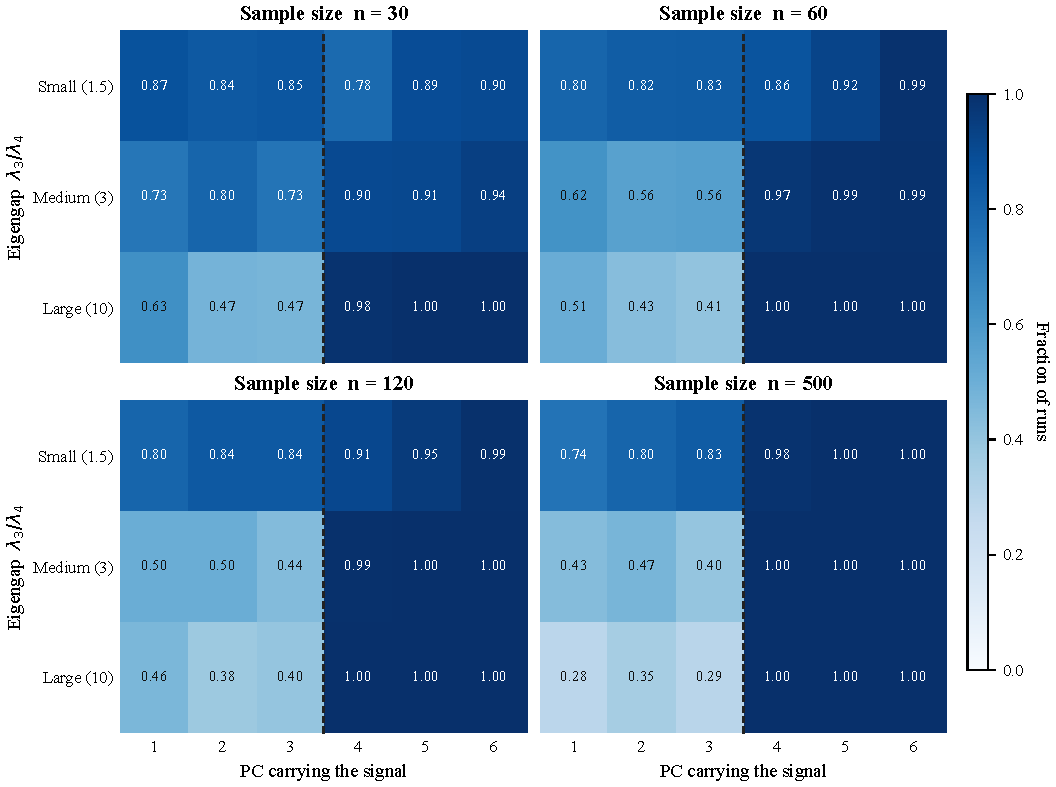
\includegraphics[width=0.82\linewidth]{../figures/fig1_disagreement_rate.pdf}
\caption{Fraction of runs in which the two rules select different ranks. Rows: eigengap size; columns: principal component carrying the signal; panels: sample size. Dashed line: position of the eigengap.}
\end{figure}

\begin{figure}[!htbp]
\centering
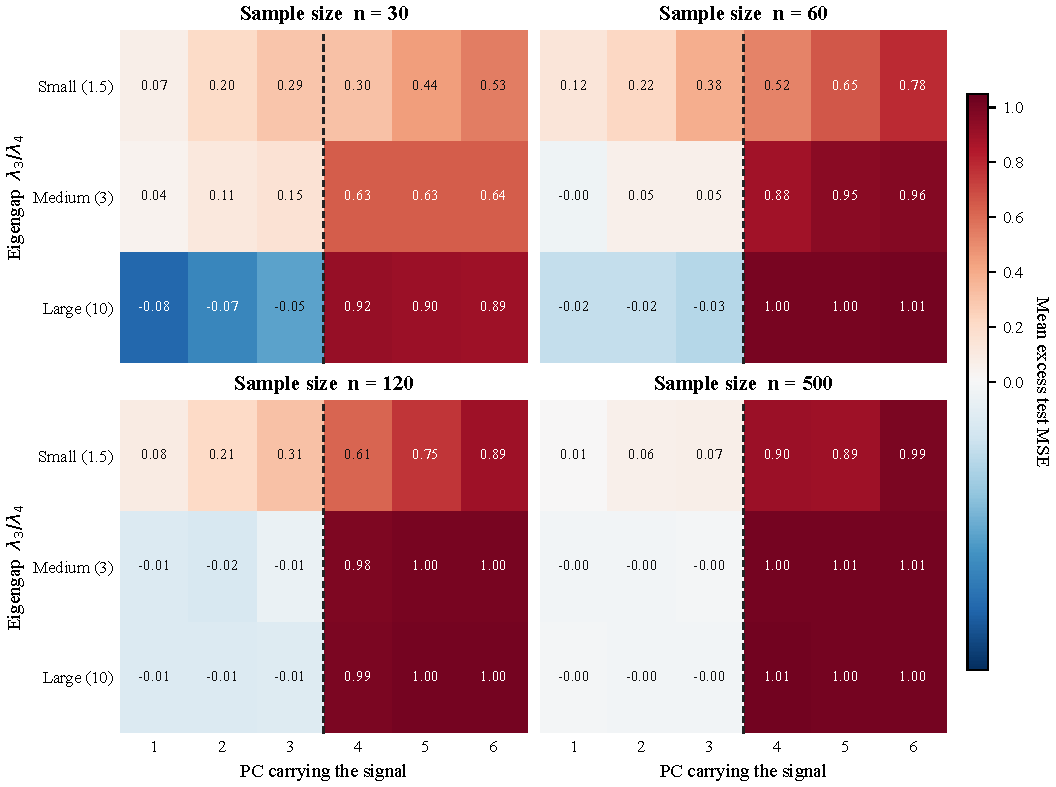
\includegraphics[width=0.82\linewidth]{../figures/fig2_test_error_cost.pdf}
\caption{Mean excess test MSE from using the stability-selected rank instead of the CV-selected rank. The signal variance is 1, so a value of 1 means the full signal is lost.}
\end{figure}

Figures 1 and 2 split cleanly at the eigengap (Table 2). Beyond the gap, disagreement approaches 100\% and its cost approaches the full signal variance. Before the gap, the methods still disagree often, because CV tends to add one or two harmless components, but the cost is small. With a large gap and $n=30$ the cost is slightly negative (-0.07): CV over-selects at small n and stability selection is marginally better.\par

\begin{table}[!htbp]
\centering
\caption{Disagreement rate and mean $\Delta$, averaged over the three signal locations on each side of the gap.}
\scriptsize
\setlength{\tabcolsep}{3.2pt}
\begin{tabular}{@{}lrrrrrrrrr@{}}
\toprule
Signal & Gap & Disagree n=30 & 60 & 120 & 500 & $\Delta$ n=30 & 60 & 120 & 500 \\
\midrule
before & small & 0.86 & 0.82 & 0.82 & 0.79 & 0.19 & 0.24 & 0.20 & 0.04 \\
before & medium & 0.75 & 0.58 & 0.48 & 0.43 & 0.10 & 0.03 & -0.01 & 0.00 \\
before & large & 0.52 & 0.45 & 0.41 & 0.31 & -0.07 & -0.03 & -0.01 & 0.00 \\
beyond & small & 0.85 & 0.92 & 0.95 & 1.00 & 0.43 & 0.65 & 0.75 & 0.92 \\
beyond & medium & 0.92 & 0.98 & 1.00 & 1.00 & 0.64 & 0.93 & 0.99 & 1.01 \\
beyond & large & 1.00 & 1.00 & 1.00 & 1.00 & 0.90 & 1.00 & 1.00 & 1.01 \\
\bottomrule
\end{tabular}
\end{table}

The consequence is that disagreement rate alone is a misleading summary. The same disagreement rate (for example about 0.8) can mean almost no loss (signal before a small gap, $n=500$) or a large loss (signal beyond the gap). Cost must be reported alongside disagreement.\par

\subsection{The main pattern: stability up, prediction down}

Table 4 shows how often stability selection recovers the structural rank $k=3$. It rises with both eigengap and sample size, as subspace theory predicts. Reading Table 4 against the 'beyond' rows of Table 2 gives the central result: in exactly the conditions where stability selection becomes reliable, its predictive loss beyond the gap becomes total and consistent. With a large gap and $n\geq 60$, $\Delta$ exceeded 0.5 (more than half the signal variance lost) in 99.9\% of beyond-the-gap runs, exceeded 0.9 in 89.8\%, and averaged 1.00. With a small gap, stability selection is erratic, occasionally picks $k=5$ by chance and so recovers part of the signal; its average loss is smaller (0.43 at $n=30$) only because it is less reliable.\par

Table 3 separates the signal locations where the candidate-rank asymmetry matters. For PC 4--5, both rules can select a rank that retains the signal ($k\geq j$ is available to stability selection), yet with a large gap stability selection retained it in 0\% of runs at every n, and $\Delta$ exceeded 0.5 in 99.9\% of runs with $n\geq 60$ (mean $\Delta=1.00$). The main pattern is therefore driven by the eigengap, not by the excluded rank. With a small gap, stability selection retained a PC 4--5 signal in 32--41\% of runs for $n\leq 120$, which is exactly why its average loss is lower there. For PC 6, retention is impossible by construction (0\% in every condition), and the effect of the restriction is visible only in the small-gap row, where the loss is higher than for PC 4--5 (for example 0.53 vs 0.37 at $n=30$). The residual gap from 1.0 in that row reflects sample principal directions mixing PC 6 into the estimated top-5 subspace when trailing eigenvalues are close.\par

\begin{table}[!htbp]
\centering
\caption{Beyond-the-gap results split by whether stability selection can retain the signal. $\Delta$: mean excess test MSE. Retained: fraction of runs with $k_{\mathrm{stability}}$ $\geq$ j.}
\scriptsize
\setlength{\tabcolsep}{3.2pt}
\begin{tabular}{@{}lrrrrrrrrr@{}}
\toprule
Signal & Gap & $\Delta$ n=30 & 60 & 120 & 500 & Retained n=30 & 60 & 120 & 500 \\
\midrule
PC 4--5 & small & 0.37 & 0.59 & 0.68 & 0.89 & 0.41 & 0.40 & 0.32 & 0.10 \\
PC 4--5 & medium & 0.63 & 0.91 & 0.99 & 1.00 & 0.18 & 0.08 & 0.01 & 0.00 \\
PC 4--5 & large & 0.91 & 1.00 & 1.00 & 1.01 & 0.00 & 0.00 & 0.00 & 0.00 \\
PC 6 & small & 0.53 & 0.78 & 0.89 & 0.99 & 0.00 & 0.00 & 0.00 & 0.00 \\
PC 6 & medium & 0.64 & 0.96 & 1.00 & 1.01 & 0.00 & 0.00 & 0.00 & 0.00 \\
PC 6 & large & 0.89 & 1.01 & 1.00 & 1.00 & 0.00 & 0.00 & 0.00 & 0.00 \\
\bottomrule
\end{tabular}
\end{table}

\begin{table}[!htbp]
\centering
\caption{Fraction of runs in which stability selection chooses the structural rank $k=3$ (all signal locations pooled; stability selection does not use y).}
\scriptsize
\setlength{\tabcolsep}{3.2pt}
\begin{tabular}{@{}lrrrr@{}}
\toprule
Eigengap & $n=30$ & $n=60$ & $n=120$ & $n=500$ \\
\midrule
small (1.5) & 0.06 & 0.10 & 0.26 & 0.80 \\
medium (3) & 0.37 & 0.78 & 0.98 & 1.00 \\
large (10) & 0.97 & 1.00 & 1.00 & 1.00 \\
\bottomrule
\end{tabular}
\end{table}

\subsection{Why the reliability changes: subspace perturbation}

\begin{figure}[!htbp]
\centering
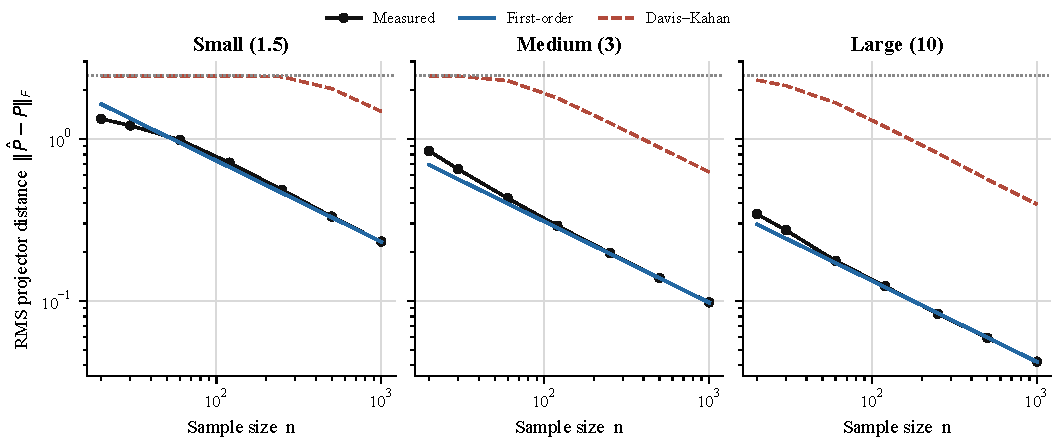
\includegraphics[width=0.92\linewidth]{../figures/fig3_subspace_distance.pdf}
\caption{Root-mean-square distance between the estimated and true top-3 subspace projectors (500 samples per point). Solid: first-order approximation; dashed: Davis--Kahan bound; dotted: the maximum possible distance $\sqrt{6}$.}
\end{figure}

Figure 3 explains Table 4. Measured instability falls like $1/\sqrt{n}$ and scales inversely with the gap. The first-order approximation tracks the measurements to within 5\% for $n\geq 250$ at every gap, and to within about 7\% from $n=60$ (medium and large gaps) or $n=120$ (small gap). Below that it overestimates, because the true distance is capped at $\sqrt{6}$. The Davis--Kahan bound is always valid but 5--10 times looser, and for the small gap it is uninformative (saturated at $\sqrt{6}$) up to n $\approx$ 250. It explains the direction of the effect, not its size.\par

\section{Discussion}

Stability selection measures how well the data determine a subspace; it says nothing about whether that subspace contains the predictive signal. Both facts are elementary. What the experiment adds is the shape of their interaction: the confidence of a stability-based choice (large gap, large n) is not evidence of predictive adequacy, and in this setting it is the condition under which the method fails predictively with near certainty when the signal lies past the gap. Stated as specifically as the evidence allows: in a controlled six-dimensional regression study, stronger eigenvalue separation made bootstrap-based PCA rank selection more consistent, but also made its predictive failure more systematic when the regression signal lay outside the selected subspace, and the resulting excess test error was approximately equal to the variance of the discarded signal. A practical reading is that, when PCR is used for prediction, a confidently stable rank should still be checked by CV, or the discarded components should be tested for association with y before being dropped.\par

\section{Limitations}

\begin{itemize}

\item The signal lies exactly along one principal direction. Real signals are mixtures across components; mixed signals would likely blur the sharp boundary.

\item The candidate ranks differ (\{1, \ldots{}, 5\} for stability, \{1, \ldots{}, 6\} for CV), so stability selection cannot retain a PC 6 signal by construction. The main conclusions are stated for PC 4--5, where this restriction does not apply (Table 3).

\item A single gap position (after component 3), one spectrum family, and $p=6$.

\item SNR fixed at 1 in the main grid (varied only in the Table 1 check).

\item $B=50$ bootstrap resamples and one stability criterion; the exact criteria of Besse (1992) and Song \& Shin (2018) were not implemented.

\item Only supervised CV was compared. Unsupervised CV of PCA (Wold, 1978; Bro et al., 2008) would ignore y and is expected to side with stability selection.

\item Gaussian data only; heavy tails would affect both subspace stability and the approximation in Figure 3.

\end{itemize}

\section{Reproducibility and next steps}

All results come from experiment.py (generator, both selectors, 72-condition grid), checks.py (Section 3), split\_analysis.py (Table 3) and plots.py (figures), with outputs results.csv, beyond\_gap\_split.csv, results\_geometric\_pilot.csv, subspace\_distance.csv and checks\_output.txt. The full grid runs in about two minutes on a laptop CPU.\par

\textbf{Literature check.} Stability-based rank selection (Besse, 1992; Song \& Shin, 2018), cross-validated PCR rank selection (Shin \& Tanaka, 1996), and the predictive failure of variance-ordered component selection (Jolliffe, 1982; Hadi \& Ling, 1998; Artigue \& Smith, 2019, including Monte Carlo evidence) are all established. No prior study found in this check compares the two selection rules directly while jointly controlling eigengap, signal location and sample size, but that check was not exhaustive, so the result is presented as a reproducible empirical characterisation rather than a verified novel finding.\par

\section*{References}

\hangindent=1.5em\hangafter=1 Anderson, T. W. (1963). Asymptotic theory for principal component analysis. Annals of Mathematical Statistics, 34(1), 122--148.\par

\hangindent=1.5em\hangafter=1 Artigue, H., \& Smith, G. (2019). The principal problem with principal components regression. Cogent Mathematics \& Statistics, 6(1), 1622190. https://doi.org/10.1080/25742558.2019.1622190\par

\hangindent=1.5em\hangafter=1 Besse, P. (1992). PCA stability and choice of dimensionality. Statistics \& Probability Letters, 13(5), 405--410.\par

\hangindent=1.5em\hangafter=1 Bro, R., Kjeldahl, K., Smilde, A. K., \& Kiers, H. A. L. (2008). Cross-validation of component models: a critical look at current methods. Analytical and Bioanalytical Chemistry, 390, 1241--1251.\par

\hangindent=1.5em\hangafter=1 Davis, C., \& Kahan, W. M. (1970). The rotation of eigenvectors by a perturbation. III. SIAM Journal on Numerical Analysis, 7(1), 1--46.\par

\hangindent=1.5em\hangafter=1 Hadi, A. S., \& Ling, R. F. (1998). Some cautionary notes on the use of principal components regression. The American Statistician, 52(1), 15--19.\par

\hangindent=1.5em\hangafter=1 Jolliffe, I. T. (1982). A note on the use of principal components in regression. Applied Statistics, 31(3), 300--303.\par

\hangindent=1.5em\hangafter=1 Shin, J. K., \& Tanaka, Y. (1996). Cross-validatory choice for the number of principal components in principal component regression. Journal of the Japanese Society of Computational Statistics, 9, 53--59.\par

\hangindent=1.5em\hangafter=1 Song, J., \& Shin, S. J. (2018). Stability approach to selecting the number of principal components. Computational Statistics, 33(4), 1923--1938. https://doi.org/10.1007/s00180-018-0826-7\par

\hangindent=1.5em\hangafter=1 Wold, S. (1978). Cross-validatory estimation of the number of components in factor and principal components models. Technometrics, 20(4), 397--405.\par

\hangindent=1.5em\hangafter=1 Yu, Y., Wang, T., \& Samworth, R. J. (2015). A useful variant of the Davis--Kahan theorem for statisticians. Biometrika, 102(2), 315--323.\par
\end{document}
